
The general equation of a second degree can be expressed as: 
\begin{align}
   \vec{x}^T\vec{V}\vec{x}+2\vec{u}^T\vec{x}+f=0
\end{align}
Comparing 1.0.1 with 2.0.1
\begin{align}
  \vec{V}=\vec{I}, \vec{u}=\myvec{\frac{-7}{2}\\\frac{-5}{2}}, f=18
\end{align}
The vector equation of a line can be expressed as  
\begin{align}
\vec{x}=\vec{q}+ \mu \vec{m}
\end{align}
{Tangent-1} Given point
\begin{align}
\vec{q_1}=\myvec{4\\3}
\end{align}
The direction vector of the line joining the point $\vec{q_1}$ and the centre $\vec{c}$ expressed as:
\begin{align}
 \vec{n_1}=\vec{q_1}-\vec{c}
 \end{align}
\begin{align}
\implies \vec{n_1}=\vec{q_1}+\vec{u}      
\end{align}
where, 
\begin{align}
\vec{c}=-\vec{u} 
\end{align}
The vector $\vec{n_1}$ is normal to the tangent drawn at $\vec{q_1}$. 
From (2.0.2) and (2.1.1) we get,
\begin{align}
\vec{n_1}^T=\myvec{\frac{1}{2} & \frac{1}{2}}
\end{align}
We know,
\begin{align}
\vec{m}^T\vec{n_1} = 0
\end{align}
\begin{align}
\implies \vec{m}^T\myvec{\frac{1}{2}\\ \frac{1}{2}} = 0
\end{align}
\begin{align}
\implies \vec{m}^T= \myvec{\frac{-1}{2} & \frac{1}{2}}
\end{align}
If $\vec{q_1}$ be a point on the line and $\vec{n_1}$ is the normal vector then
the equation of the line can be expressed From(2.0.3) is :
\begin{align}
 \vec{n_1}^T (\vec{x}-\vec{q_1})=0
\end{align}
\begin{align}
 \implies \vec{n_1}^T \vec{x}= c
\end{align}
where
\begin{align}
 c=\vec{n_1}^T \vec{q_1}
\end{align}
Using the equations (2.1.1) and (2.1.5),
\begin{align}
 \implies c=\myvec{\frac{1}{2} & \frac{1}{2}} \myvec{4\\3}= \frac{7}{2}
\end{align}
From (2.1.10), Line equation of Tangent-1 is:
\begin{align}
 \myvec{\frac{1}{2} & \frac{1}{2}} \vec{x}= \frac{7}{2}
\end{align}
\begin{align}
  \implies \boxed{\myvec{1 & 1} \vec{x}= 7}
\end{align}
{Tangent-2} Now,
\begin{align}
\vec{q_2}=\myvec{3\\2}
\end{align}
The direction vector of the line joining the point $\vec{q_2}$ and the centre $\vec{c}$ expressed as:
\begin{align}
 \vec{n_2}=\vec{q_2}-\vec{c}
 \end{align}
 \begin{align}
 \implies \vec{n_2}=\vec{q_2}+\vec{u}
 \end{align}
 where, 
\begin{align}
\vec{c}=-\vec{u} 
\end{align}
The vector $\vec{n_2}$ is normal to the tangent drawn at $\vec{q_2}$.
From (2.0.2) and (2.2.1),
\begin{align}
\vec{n_2}^T=\myvec{\frac{-1}{2} & \frac{-1}{2}}
\end{align}
We know,
\begin{align}
\vec{m}^T\vec{n_2} = 0
\end{align}
\begin{align}
\implies \vec{m}^T\myvec{\frac{-1}{2}\\ \frac{-1}{2}} = 0
\end{align}
\begin{align}
\implies \vec{m}^T= \myvec{\frac{1}{2} & \frac{-1}{2}}
\end{align}
If $\vec{q_2}$ be a point on the line and $\vec{n_2}$ is the normal vector, the equation of the line can be expressed From (2.0.3) is:
\begin{align}
 \vec{n_2}^T (\vec{x}-\vec{q_2})=0
\end{align}
\begin{align}
 \implies \vec{n_2}^T \vec{x}= c
\end{align}
where
\begin{align}
 c=\vec{n_2}^T \vec{q_2}
\end{align}
Using the equations 2.2.1 and 2.2.5,
\begin{align}
 \implies c=\myvec{\frac{-1}{2} & \frac{-1}{2}} \myvec{3\\2}= \frac{-5}{2}
\end{align}
From (2.2.10), Line equation of Tangent-2 is:
\begin{align}
 \myvec{\frac{-1}{2} & \frac{-1}{2}} \vec{x}= \frac{-5}{2}
\end{align}
\begin{align}
  \implies \boxed {\myvec{1 & 1} \vec{x}= 5 }
\end{align}
{Result}
From the equations (2.1.14) and (2.2.14), normal vectors of Tangent-1 and Tangent-2 are equal. \newline 
\centering Hence, the two tangents are parallel.
\begin{figure}[h!]
	\centering
	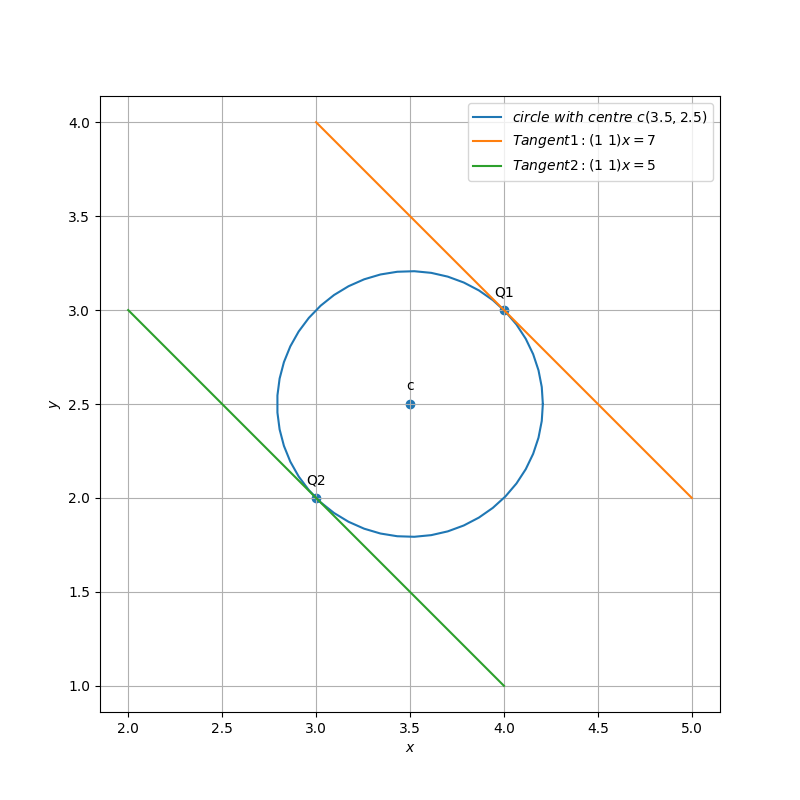
\includegraphics[width=\columnwidth]{./solutions/4/2/9/Codes/A4.png}
	\caption{Tangents to the circle at given points}
	\label{eq:solutions/4/2/9/myfig}
\end{figure}
